\documentclass{article}

\usepackage{pdfpages}                 % to include the cover sheet as the first page
\usepackage[margin=1in]{geometry}
                                      %for 1inch margins that play nice with fancyhdr
\usepackage{amsmath,amssymb}          % math and junk
\usepackage{fancyhdr}                 % for a nice running header and footer
\usepackage{lastpage}                 % for nice "X of Y" footer
\usepackage[per-mode=symbol]{siunitx} % for nice units and junk!
\usepackage{gnuplot-lua-tikz}         % enable tikz plots made from gnuplot
\usepackage{float}                    % [H] option for floats
\usepackage[american]{circuitikz}     % for teh circuit diagrams

% unused, but common for other experiments
%\usepackage{rotating}                 % for sideways stuff!
%\usepackage{cancel}                   % for `canceling out' parts of equations. fancy!
%\usepackage{mdwlist}                  % itemize* and friends
%\usepackage{verbatim}                 % for \verbatiminput command and comment environment
%\usepackage[colorinlistoftodos]{todonotes}                % todo's, if used/needed
%\usepackage{multirow}                 % for multi-row spans in tabular environment


% for fancy header
\pagestyle{fancy}
\lhead{ECE-L303 Section 062}
\chead{Lab 1: Electronic Devices}
\rhead{Sean Barag}
\cfoot{\thepage\ of \pageref{LastPage}}

% title info
\title{ECE-L303 Lab 1: \\ Electronic Devices}
\author{Sean Barag \\ Lab Partners: None}
\date{}

% shortcuts, cause I'm lazy
\newcommand{\bs}[1]{\boldsymbol{#1}}
\newcommand{\tbf}[1]{\textbf{#1}}

\begin{document}
% Cover page to appease Dr. Gerber/Miu
\includepdf{../../coverSheet.pdf}

% Blank page so two-sided printing leaves the cover page on its own sheet
\thispagestyle{empty}
\newpage
\mbox{}

\maketitle
\setcounter{page}{1} % fixes page numbering issues caused by cover sheet
\tableofcontents % this helps

\newpage % I want object to be at the top of a new page
\section{Object}
The object of experiment seven was to provide students with valuable information on the construction and function of a voltage-controlled oscillator (VCO).  Additionally, students were give the opportunity to design the experiment performed within.


\section{Circuit Diagrams}
\begin{figure}[H]
	\centering
	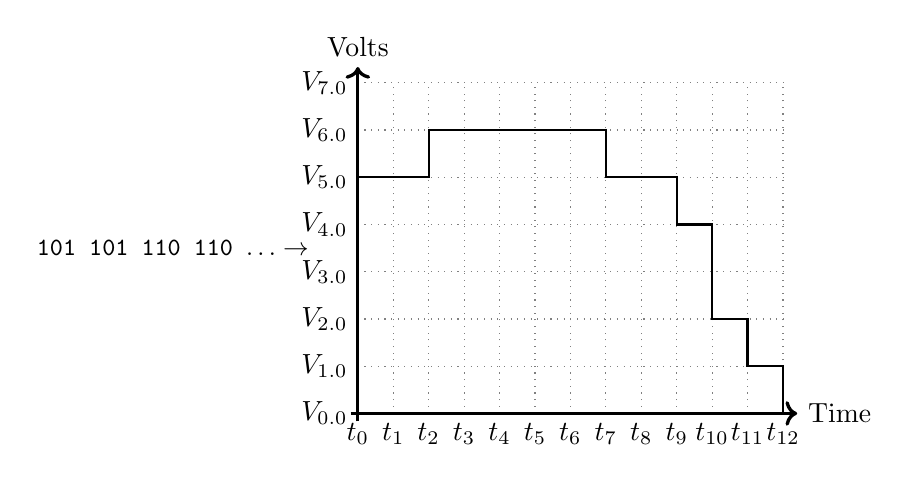
\begin{tikzpicture}[xscale=.9]
		% samples
		\draw[xstep=.5, ystep=.6, thin, color=gray, dotted] (0,0) grid (6, 4.2);

		% path
		\draw[thick]
		(0, 3)
		-- (.5, 3) -- (1, 3)
		-- (1, 3.6) -- (1.5, 3.6) -- (2, 3.6) -- (2.5, 3.6) -- (3, 3.6) -- (3.5, 3.6)
		-- (3.5, 3) -- (4, 3) -- (4.5, 3)
		-- (4.5, 2.4) -- (5, 2.4)
		-- (5, 1.2) -- (5.5, 1.2)
		-- (5.5, 0.6) -- (6.0, 0.6)
		-- (6.0, 0);

		% xtics
		\foreach \x in {0, ..., 12}
		{
			\draw ({\x/2}, 0) node[below] {$t_{\x}$};
		}

		% ytics
		\foreach \y in {0, 1, ..., 7.1}
		{
			\draw[thick] (0, .6*\y) node[left] {$V_{\num[round-mode=places, round-precision=1]{\y}}$};
		}

		% axes
    	\draw[->, very thick] (-0.1,0) -- (6.2,0) node[right] {Time};
    	\draw[->, very thick] (0,-.1) -- (0,4.4) node[above] {Volts};

		% data input
		\draw
		(0, 2.1) node[left=.5cm]{\texttt{\small 101 101 110 110 $\ldots \rightarrow$}};
\end{tikzpicture}

\end{figure}

\begin{figure}[H]
	\centering
	\begin{circuitikz}
	\tikzstyle{leftPin}  = [anchor=west]
	\tikzstyle{rightPin} = [left]

	% body
	\draw[ultra thick] (-2, -4) rectangle (2, 4);

	% left pins

	% right pins
	\foreach \y in {7, ..., 0}
	{
		\draw (2, \y-3.5) node[rightPin] (b\y) {B\y}
		to [short] ++(.5,0) to [R, l=$R$] ++(1.5,0)
		++(1.5, 0) to [led, *-] ++(-1.5, 0);
	}

	\foreach \pin in {11,...,18}
	{
		\draw (2, 14.5-\pin) node[above right] {\pin};
	}

	\draw (b7) node[left=4pt] {MSB}
	(b0) node[left=4pt] {LSB};

	% 5V rail
	\draw (5.5, -3.5) to [short] ++(0, 8.5) node[above] {\SI{5.2}{\volt}};

	\draw (0, 4) node[above left] {20} to [short] ++(0, 2) coordinate (top junc) to [short] ++(1, 0)
	to [C, l=$C_4$: \SI{10}{\micro\farad}] ++(0, -1) node[ground] {}
	(top junc) to [short] ++(0, .5) node[above] {\SI{5.12}{\volt}};

	% left pins

\end{circuitikz}

\end{figure}

\begin{figure}[H]
	\centering
	\input{img/pt4bars.tex}
\end{figure}

\begin{figure}[H]
	\centering
	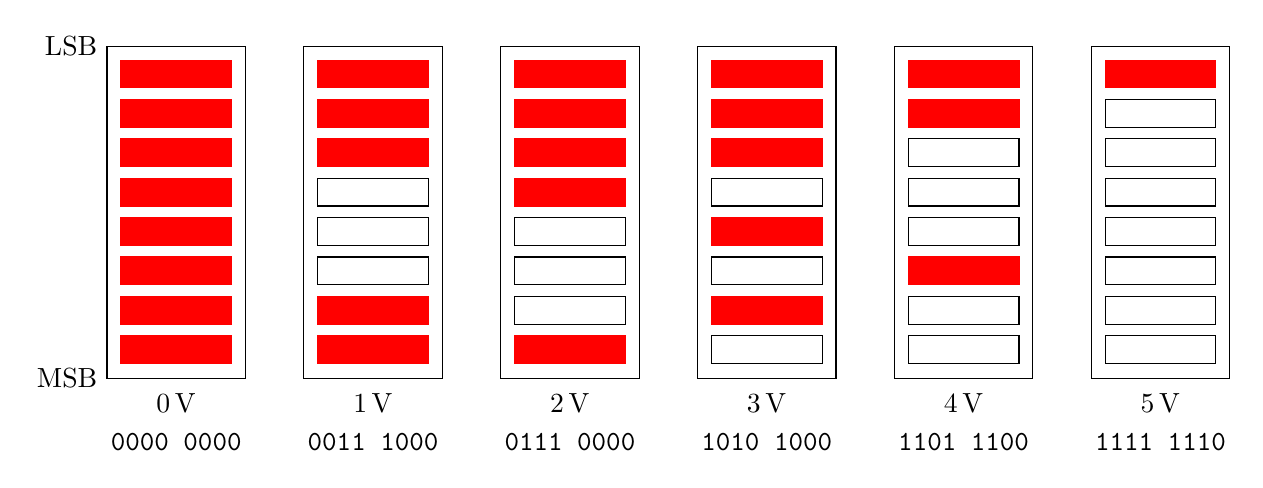
\begin{tikzpicture}[node distance=.5cm, auto, >=latex']
   \tikzstyle{off}=[rectangle, draw, minimum width=4em, minimum height=1em]
   \tikzstyle{on} =[rectangle, draw=red, fill=red, minimum width=4em, minimum height=1em]

   % bar one
   \begin{scope}
   	% outer box
   	\draw (-2.5em,1em) rectangle (2.5em,-11em);

   	% labels -- ONLY DO THESE ONCE
   	\draw (-2.5em, 1em) node[left] {LSB};
   	\draw (-2.5em,-11em) node[left] {MSB};

   	% led bars
   	\node[on] (bit0) {};
   	\node[on,  below of=bit0] (bit1) {};
   	\node[on,  below of=bit1] (bit2) {};
   	\node[on, below of=bit2] (bit3) {};

   	\node[on, below of=bit3] (bit4) {};
   	\node[on, below of=bit4] (bit5) {};
   	\node[on, below of=bit5] (bit6) {};
   	\node[on,  below of=bit6] (bit7) {};

   	% voltage
   	\node[below of=bit7, yshift=-.5em] (voltage) {\SI{0}{\volt}};

   	% bit mask
   	\node[below of=voltage] (bitMask) {\texttt{0000 0000}};
   \end{scope}

   \begin{scope}[xshift = 2.5cm]
   	% outer box
   	\draw (-2.5em,1em) rectangle (2.5em,-11em);

   	% led bars
   	\node[on] (bit0) {};
   	\node[on, below of=bit0] (bit1) {};
   	\node[on,  below of=bit1] (bit2) {};
   	\node[off,  below of=bit2] (bit3) {};

   	\node[off, below of=bit3] (bit4) {};
   	\node[off, below of=bit4] (bit5) {};
   	\node[on,  below of=bit5] (bit6) {};
   	\node[on,  below of=bit6] (bit7) {};

   	% voltage
   	\node[below of=bit7, yshift=-.5em] (voltage) {\SI{1}{\volt}};

   	% bit mask
   	\node[below of=voltage] (bitMask) {\texttt{0011 1000}};
   \end{scope}

   \begin{scope}[xshift = 5cm]
   	% outer box
   	\draw (-2.5em,1em) rectangle (2.5em,-11em);

   	% led bars
   	\node[on] (bit0) {};
   	\node[on, below of=bit0] (bit1) {};
   	\node[on, below of=bit1] (bit2) {};
   	\node[on,  below of=bit2] (bit3) {};

   	\node[off,  below of=bit3] (bit4) {};
   	\node[off, below of=bit4] (bit5) {};
   	\node[off, below of=bit5] (bit6) {};
   	\node[on,  below of=bit6] (bit7) {};

   	% voltage
   	\node[below of=bit7, yshift=-.5em] (voltage) {\SI{2}{\volt}};

   	% bit mask
   	\node[below of=voltage] (bitMask) {\texttt{0111 0000}};
   \end{scope}

   \begin{scope}[xshift = 7.5cm]
   	% outer box
   	\draw (-2.5em,1em) rectangle (2.5em,-11em);

   	% led bars
   	\node[on] (bit0) {};
   	\node[on,  below of=bit0] (bit1) {};
   	\node[on, below of=bit1] (bit2) {};
   	\node[off, below of=bit2] (bit3) {};

   	\node[on, below of=bit3] (bit4) {};
   	\node[off, below of=bit4] (bit5) {};
   	\node[on,  below of=bit5] (bit6) {};
   	\node[off,  below of=bit6] (bit7) {};

   	% voltage
   	\node[below of=bit7, yshift=-.5em] (voltage) {\SI{3}{\volt}};

   	% bit mask
   	\node[below of=voltage] (bitMask) {\texttt{1010 1000}};
   \end{scope}

   \begin{scope}[xshift = 10cm]
   	% outer box
   	\draw (-2.5em,1em) rectangle (2.5em,-11em);

   	% led bars
   	\node[on] (bit0) {};
   	\node[on,  below of=bit0] (bit1) {};
   	\node[off, below of=bit1] (bit2) {};
   	\node[off, below of=bit2] (bit3) {};

   	\node[off,  below of=bit3] (bit4) {};
   	\node[on,  below of=bit4] (bit5) {};
   	\node[off, below of=bit5] (bit6) {};
   	\node[off, below of=bit6] (bit7) {};

   	% voltage
   	\node[below of=bit7, yshift=-.5em] (voltage) {\SI{4}{\volt}};

   	% bit mask
   	\node[below of=voltage] (bitMask) {\texttt{1101 1100}};
   \end{scope}

   \begin{scope}[xshift = 12.5cm]
   	% outer box
   	\draw (-2.5em,1em) rectangle (2.5em,-11em);

   	% led bars
   	\node[on] (bit0) {};
   	\node[off,  below of=bit0] (bit1) {};
   	\node[off,  below of=bit1] (bit2) {};
   	\node[off, below of=bit2] (bit3) {};

   	\node[off,  below of=bit3] (bit4) {};
   	\node[off, below of=bit4] (bit5) {};
   	\node[off, below of=bit5] (bit6) {};
   	\node[off, below of=bit6] (bit7) {};

   	% voltage
   	\node[below of=bit7, yshift=-.5em] (voltage) {\SI{5}{\volt}};

   	% bit mask
   	\node[below of=voltage] (bitMask) {\texttt{1111 1110}};
   \end{scope}

\end{tikzpicture}

\end{figure}

\begin{figure}[H]
	\centering
	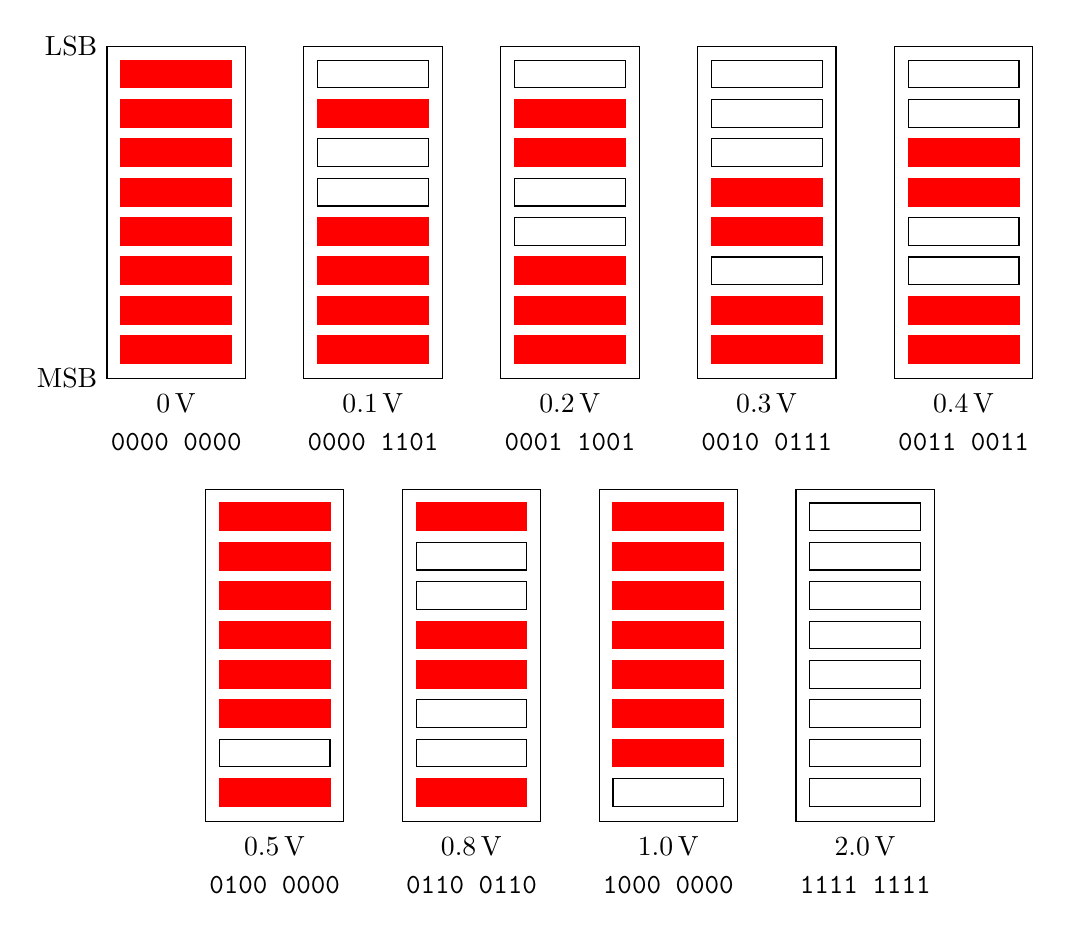
\begin{tikzpicture}[node distance=.5cm, auto, >=latex']
   \tikzstyle{off}=[rectangle, draw, minimum width=4em, minimum height=1em]
   \tikzstyle{on} =[rectangle, draw=red, fill=red, minimum width=4em, minimum height=1em]

   % bar one
   \begin{scope}
   	% outer box
   	\draw (-2.5em,1em) rectangle (2.5em,-11em);

   	% labels -- ONLY DO THESE ONCE
   	\draw (-2.5em, 1em) node[left] {LSB};
   	\draw (-2.5em,-11em) node[left] {MSB};

   	% led bars
   	\node[on] (bit0) {};
   	\node[on,  below of=bit0] (bit1) {};
   	\node[on,  below of=bit1] (bit2) {};
   	\node[on, below of=bit2] (bit3) {};

   	\node[on, below of=bit3] (bit4) {};
   	\node[on, below of=bit4] (bit5) {};
   	\node[on, below of=bit5] (bit6) {};
   	\node[on,  below of=bit6] (bit7) {};

   	% voltage
   	\node[below of=bit7, yshift=-.5em] (voltage) {\SI{0}{\volt}};

   	% bit mask
   	\node[below of=voltage] (bitMask) {\texttt{0000 0000}};
   \end{scope}

   \begin{scope}[xshift = 2.5cm]
   	% outer box
   	\draw (-2.5em,1em) rectangle (2.5em,-11em);

   	% led bars
   	\node[off] (bit0) {};
   	\node[on, below of=bit0] (bit1) {};
   	\node[off,  below of=bit1] (bit2) {};
   	\node[off,  below of=bit2] (bit3) {};

   	\node[on, below of=bit3] (bit4) {};
   	\node[on, below of=bit4] (bit5) {};
   	\node[on,  below of=bit5] (bit6) {};
   	\node[on,  below of=bit6] (bit7) {};

   	% voltage
   	\node[below of=bit7, yshift=-.5em] (voltage) {\SI{0.1}{\volt}};

   	% bit mask
   	\node[below of=voltage] (bitMask) {\texttt{0000 1101}};
   \end{scope}

   \begin{scope}[xshift = 5cm]
   	% outer box
   	\draw (-2.5em,1em) rectangle (2.5em,-11em);

   	% led bars
   	\node[off] (bit0) {};
   	\node[on, below of=bit0] (bit1) {};
   	\node[on, below of=bit1] (bit2) {};
   	\node[off,  below of=bit2] (bit3) {};

   	\node[off,  below of=bit3] (bit4) {};
   	\node[on, below of=bit4] (bit5) {};
   	\node[on, below of=bit5] (bit6) {};
   	\node[on,  below of=bit6] (bit7) {};

   	% voltage
   	\node[below of=bit7, yshift=-.5em] (voltage) {\SI{0.2}{\volt}};

   	% bit mask
   	\node[below of=voltage] (bitMask) {\texttt{0001 1001}};
   \end{scope}

   \begin{scope}[xshift = 7.5cm]
   	% outer box
   	\draw (-2.5em,1em) rectangle (2.5em,-11em);

   	% led bars
   	\node[off] (bit0) {};
   	\node[off,  below of=bit0] (bit1) {};
   	\node[off, below of=bit1] (bit2) {};
   	\node[on, below of=bit2] (bit3) {};

   	\node[on, below of=bit3] (bit4) {};
   	\node[off, below of=bit4] (bit5) {};
   	\node[on,  below of=bit5] (bit6) {};
   	\node[on,  below of=bit6] (bit7) {};

   	% voltage
   	\node[below of=bit7, yshift=-.5em] (voltage) {\SI{0.3}{\volt}};

   	% bit mask
   	\node[below of=voltage] (bitMask) {\texttt{0010 0111}};
   \end{scope}

   \begin{scope}[xshift = 10cm]
   	% outer box
   	\draw (-2.5em,1em) rectangle (2.5em,-11em);

   	% led bars
   	\node[off] (bit0) {};
   	\node[off,  below of=bit0] (bit1) {};
   	\node[on, below of=bit1] (bit2) {};
   	\node[on, below of=bit2] (bit3) {};

   	\node[off,  below of=bit3] (bit4) {};
   	\node[off,  below of=bit4] (bit5) {};
   	\node[on, below of=bit5] (bit6) {};
   	\node[on, below of=bit6] (bit7) {};

   	% voltage
   	\node[below of=bit7, yshift=-.5em] (voltage) {\SI{0.4}{\volt}};

   	% bit mask
   	\node[below of=voltage] (bitMask) {\texttt{0011 0011}};
   \end{scope}

   \begin{scope}[xshift = 1.25cm, yshift=-16em]
   	% outer box
   	\draw (-2.5em,1em) rectangle (2.5em,-11em);

   	% led bars
   	\node[on] (bit0) {};
   	\node[on,  below of=bit0] (bit1) {};
   	\node[on,  below of=bit1] (bit2) {};
   	\node[on, below of=bit2] (bit3) {};

   	\node[on,  below of=bit3] (bit4) {};
   	\node[on, below of=bit4] (bit5) {};
   	\node[off, below of=bit5] (bit6) {};
   	\node[on, below of=bit6] (bit7) {};

   	% voltage
   	\node[below of=bit7, yshift=-.5em] (voltage) {\SI{0.5}{\volt}};

   	% bit mask
   	\node[below of=voltage] (bitMask) {\texttt{0100 0000}};
   \end{scope}

   \begin{scope}[xshift = 3.75cm, yshift=-16em]
   	% outer box
   	\draw (-2.5em,1em) rectangle (2.5em,-11em);

   	% led bars
   	\node[on] (bit0) {};
   	\node[off,  below of=bit0] (bit1) {};
   	\node[off,  below of=bit1] (bit2) {};
   	\node[on, below of=bit2] (bit3) {};

   	\node[on,  below of=bit3] (bit4) {};
   	\node[off, below of=bit4] (bit5) {};
   	\node[off, below of=bit5] (bit6) {};
   	\node[on, below of=bit6] (bit7) {};

   	% voltage
   	\node[below of=bit7, yshift=-.5em] (voltage) {\SI{0.8}{\volt}};

   	% bit mask
   	\node[below of=voltage] (bitMask) {\texttt{0110 0110}};
   \end{scope}

   \begin{scope}[xshift = 6.25cm, yshift=-16em]
   	% outer box
   	\draw (-2.5em,1em) rectangle (2.5em,-11em);

   	% led bars
   	\node[on] (bit0) {};
   	\node[on,  below of=bit0] (bit1) {};
   	\node[on,  below of=bit1] (bit2) {};
   	\node[on, below of=bit2] (bit3) {};

   	\node[on,  below of=bit3] (bit4) {};
   	\node[on, below of=bit4] (bit5) {};
   	\node[on, below of=bit5] (bit6) {};
   	\node[off, below of=bit6] (bit7) {};

   	% voltage
   	\node[below of=bit7, yshift=-.5em] (voltage) {\SI{1.0}{\volt}};

   	% bit mask
   	\node[below of=voltage] (bitMask) {\texttt{1000 0000}};
   \end{scope}

   \begin{scope}[xshift = 8.75cm, yshift=-16em]
   	% outer box
   	\draw (-2.5em,1em) rectangle (2.5em,-11em);

   	% led bars
   	\node[off] (bit0) {};
   	\node[off,  below of=bit0] (bit1) {};
   	\node[off,  below of=bit1] (bit2) {};
   	\node[off, below of=bit2] (bit3) {};

   	\node[off,  below of=bit3] (bit4) {};
   	\node[off, below of=bit4] (bit5) {};
   	\node[off, below of=bit5] (bit6) {};
   	\node[off, below of=bit6] (bit7) {};

   	% voltage
   	\node[below of=bit7, yshift=-.5em] (voltage) {\SI{2.0}{\volt}};

   	% bit mask
   	\node[below of=voltage] (bitMask) {\texttt{1111 1111}};
   \end{scope}

\end{tikzpicture}

\end{figure}


\section{Data Sheet}
\subsection{Rectifier}
The half wave rectifier was buit according to the provided schematic (recreated
in Figure~\ref{fig:schem1}, where the value of the resistor was provided
as~\SI{1}{\kilo\ohm} in the instructions.  The input voltage was calculated by
multiplying the specified average voltage of~\SI{5.6}{\volt}DC by~$\pi$ as
shown in Equation~\ref{eq:v_avg}.  This resulted in a peak voltage
of~\SI{17.6}{\volt}DC.
%
\begin{equation}
	V_\text{avg} = \frac{V_p}{\pi}
	\label{eq:v_avg}
\end{equation}
%
To calculate the AC signal's root-mean-square (RMS) value, the peak voltage was
then divided by~$\sqrt{2}$, as shown in Equation~\ref{eq:rms}.
%
\begin{equation}
	V_\text{RMS} = \frac{V_p}{\sqrt{2}}
	\label{eq:rms}
\end{equation}
%
The resulting calculations provided a designed input of \SI{12.2}{\volt} (RMS).
Using an oscilloscope in combination with a variac transformer, the input was
adjusted to be as close to this value as possible. Data for the half-wave
rectifier was captured by the oscilloscope.  Due to the large number of
measurements taken, it is available by request to the author.

\subsection{Logic Indicator}
\begin{figure}[H]
	\centering
	\begin{tabular}{|c|c|c|}
\hline
\tbf{Input (V)} & \tbf{Output State} & \tbf{Comment} \\ \hline
0				& Off				& ---				\\ \hline
1				& Off				& ---				\\ \hline
2				& On				& Dim				\\ \hline
3				& On				& Brighter			\\ \hline
4				& On				& Full Brightness 	\\ \hline
5				& On				& ---				\\ \hline
\end{tabular}

	\caption{Brightness observations for the circuit shown in
		Figure~\ref{fig:schem2}.}
	\label{tab:ckt2data}
\end{figure}

\subsection{Voltage Regulator}
\begin{figure}[H]
	\centering
	\begin{tabular}{|c|c|}
\hline
\tbf{Input (V)} & \tbf{Output (V)} \\ \hline
5			& 4.997  	\\ \hline
6			& 5.997  	\\ \hline
7			& 6.998  	\\ \hline
8			& 7.999  	\\ \hline
9			& 8.999  	\\ \hline
10			& 9.751  	\\ \hline
11			& 9.810  	\\ \hline
12			& 9.850  	\\ \hline
13			& 9.940  	\\ \hline
14			& 10.017 	\\ \hline
15			& 10.089 	\\ \hline
16			& 10.157 	\\ \hline
17			& 10.230 	\\ \hline
18			& 10.312 	\\ \hline
19			& 10.388 	\\ \hline
20			& 10.440 	\\ \hline
21			& 10.390 	\\ \hline
22			& 10.331 	\\ \hline
23			& 10.268 	\\ \hline
24			& 10.199 	\\ \hline
25			& 10.140 	\\ \hline
\end{tabular}

	\caption{Output measurements of the zener diode voltage
		regulator described in Figure~\ref{fig:schem3}.}
	\label{tab:ckt3data}
\end{figure}

\subsection{Constant Current Source}
\begin{figure}[H]
	\centering
	\begin{tikzpicture}[gnuplot]
%% generated with GNUPLOT 4.4p2 (Lua 5.1.4; terminal rev. 97, script rev. 96a)
%% Wed 28 Sep 2011 01:27:40 PM EDT
\gpsolidlines
\gpcolor{gp lt color border}
\gpsetlinetype{gp lt border}
\gpsetlinewidth{1.00}
\draw[gp path] (1.504,0.985)--(1.684,0.985);
\node[gp node right] at (1.320,0.985) { 3};
\draw[gp path] (1.504,1.712)--(1.684,1.712);
\node[gp node right] at (1.320,1.712) { 3.5};
\draw[gp path] (1.504,2.439)--(1.684,2.439);
\node[gp node right] at (1.320,2.439) { 4};
\draw[gp path] (1.504,3.166)--(1.684,3.166);
\node[gp node right] at (1.320,3.166) { 4.5};
\draw[gp path] (1.504,3.892)--(1.684,3.892);
\node[gp node right] at (1.320,3.892) { 5};
\draw[gp path] (1.504,4.619)--(1.684,4.619);
\node[gp node right] at (1.320,4.619) { 5.5};
\draw[gp path] (1.504,5.346)--(1.684,5.346);
\node[gp node right] at (1.320,5.346) { 6};
\draw[gp path] (1.504,0.985)--(1.504,1.165);
\node[gp node center] at (1.504,0.677) { 0.01};
\draw[gp path] (2.381,0.985)--(2.381,1.075);
\draw[gp path] (2.894,0.985)--(2.894,1.075);
\draw[gp path] (3.258,0.985)--(3.258,1.075);
\draw[gp path] (3.540,0.985)--(3.540,1.075);
\draw[gp path] (3.770,0.985)--(3.770,1.075);
\draw[gp path] (3.965,0.985)--(3.965,1.075);
\draw[gp path] (4.134,0.985)--(4.134,1.075);
\draw[gp path] (4.283,0.985)--(4.283,1.075);
\draw[gp path] (4.417,0.985)--(4.417,1.165);
\node[gp node center] at (4.417,0.677) { 0.1};
\draw[gp path] (5.293,0.985)--(5.293,1.075);
\draw[gp path] (5.806,0.985)--(5.806,1.075);
\draw[gp path] (6.170,0.985)--(6.170,1.075);
\draw[gp path] (6.453,0.985)--(6.453,1.075);
\draw[gp path] (6.683,0.985)--(6.683,1.075);
\draw[gp path] (6.878,0.985)--(6.878,1.075);
\draw[gp path] (7.047,0.985)--(7.047,1.075);
\draw[gp path] (7.196,0.985)--(7.196,1.075);
\draw[gp path] (7.329,0.985)--(7.329,1.165);
\node[gp node center] at (7.329,0.677) { 1};
\draw[gp path] (8.206,0.985)--(8.206,1.075);
\draw[gp path] (8.719,0.985)--(8.719,1.075);
\draw[gp path] (9.083,0.985)--(9.083,1.075);
\draw[gp path] (9.365,0.985)--(9.365,1.075);
\draw[gp path] (9.596,0.985)--(9.596,1.075);
\draw[gp path] (9.791,0.985)--(9.791,1.075);
\draw[gp path] (9.960,0.985)--(9.960,1.075);
\draw[gp path] (10.109,0.985)--(10.109,1.075);
\draw[gp path] (10.242,0.985)--(10.242,1.165);
\node[gp node center] at (10.242,0.677) { 10};
\draw[gp path] (1.504,5.346)--(1.504,0.985)--(10.242,0.985);
\node[gp node center,rotate=-270] at (0.246,3.165) {Measured Current, $I_{out}$ (\si{\milli\ampere})};
\node[gp node center] at (5.873,0.215) {Load Resistance, $R$ (\si{\kilo\ohm})};
\node[gp node right] at (3.712,1.627) {16V source};
\gpcolor{gp lt color 0}
\gpsetlinetype{gp lt plot 0}
\draw[gp path] (3.896,1.627)--(4.812,1.627);
\draw[gp path] (3.540,4.881)--(4.417,4.866)--(5.293,4.866)--(5.806,4.866)--(6.170,4.866)%
  --(6.453,4.881)--(6.683,4.881)--(6.878,4.881)--(7.047,4.881)--(7.196,4.881)--(7.329,4.881)%
  --(7.450,4.881)--(7.560,4.881)--(7.661,4.881)--(7.755,4.895)--(7.842,4.895)--(7.924,4.881)%
  --(8.001,4.866)--(8.073,4.837)--(8.141,4.823)--(8.206,4.823)--(8.268,4.794)--(8.327,4.721)%
  --(8.383,4.634)--(8.437,4.517)--(8.488,4.372)--(8.538,4.212)--(8.586,4.038)--(8.632,3.863)%
  --(8.676,3.674)--(8.719,3.500)--(8.761,3.325)--(8.801,3.151)--(8.840,2.991)--(8.877,2.846)%
  --(8.914,2.686)--(8.950,2.540)--(8.984,2.410)--(9.018,2.264)--(9.051,2.133)--(9.083,2.017)%
  --(9.114,1.901)--(9.145,1.785)--(9.174,1.668)--(9.203,1.566)--(9.232,1.465)--(9.260,1.377)%
  --(9.287,1.276)--(9.314,1.189)--(9.340,1.101)--(9.365,1.014);
\gpsetpointsize{4.00}
\gppoint{gp mark 1}{(3.540,4.881)}
\gppoint{gp mark 1}{(4.417,4.866)}
\gppoint{gp mark 1}{(5.293,4.866)}
\gppoint{gp mark 1}{(5.806,4.866)}
\gppoint{gp mark 1}{(6.170,4.866)}
\gppoint{gp mark 1}{(6.453,4.881)}
\gppoint{gp mark 1}{(6.683,4.881)}
\gppoint{gp mark 1}{(6.878,4.881)}
\gppoint{gp mark 1}{(7.047,4.881)}
\gppoint{gp mark 1}{(7.196,4.881)}
\gppoint{gp mark 1}{(7.329,4.881)}
\gppoint{gp mark 1}{(7.450,4.881)}
\gppoint{gp mark 1}{(7.560,4.881)}
\gppoint{gp mark 1}{(7.661,4.881)}
\gppoint{gp mark 1}{(7.755,4.895)}
\gppoint{gp mark 1}{(7.842,4.895)}
\gppoint{gp mark 1}{(7.924,4.881)}
\gppoint{gp mark 1}{(8.001,4.866)}
\gppoint{gp mark 1}{(8.073,4.837)}
\gppoint{gp mark 1}{(8.141,4.823)}
\gppoint{gp mark 1}{(8.206,4.823)}
\gppoint{gp mark 1}{(8.268,4.794)}
\gppoint{gp mark 1}{(8.327,4.721)}
\gppoint{gp mark 1}{(8.383,4.634)}
\gppoint{gp mark 1}{(8.437,4.517)}
\gppoint{gp mark 1}{(8.488,4.372)}
\gppoint{gp mark 1}{(8.538,4.212)}
\gppoint{gp mark 1}{(8.586,4.038)}
\gppoint{gp mark 1}{(8.632,3.863)}
\gppoint{gp mark 1}{(8.676,3.674)}
\gppoint{gp mark 1}{(8.719,3.500)}
\gppoint{gp mark 1}{(8.761,3.325)}
\gppoint{gp mark 1}{(8.801,3.151)}
\gppoint{gp mark 1}{(8.840,2.991)}
\gppoint{gp mark 1}{(8.877,2.846)}
\gppoint{gp mark 1}{(8.914,2.686)}
\gppoint{gp mark 1}{(8.950,2.540)}
\gppoint{gp mark 1}{(8.984,2.410)}
\gppoint{gp mark 1}{(9.018,2.264)}
\gppoint{gp mark 1}{(9.051,2.133)}
\gppoint{gp mark 1}{(9.083,2.017)}
\gppoint{gp mark 1}{(9.114,1.901)}
\gppoint{gp mark 1}{(9.145,1.785)}
\gppoint{gp mark 1}{(9.174,1.668)}
\gppoint{gp mark 1}{(9.203,1.566)}
\gppoint{gp mark 1}{(9.232,1.465)}
\gppoint{gp mark 1}{(9.260,1.377)}
\gppoint{gp mark 1}{(9.287,1.276)}
\gppoint{gp mark 1}{(9.314,1.189)}
\gppoint{gp mark 1}{(9.340,1.101)}
\gppoint{gp mark 1}{(9.365,1.014)}
\gppoint{gp mark 1}{(4.354,1.627)}
\gpcolor{gp lt color border}
\node[gp node right] at (3.712,1.319) {32V source };
\gpcolor{gp lt color 1}
\gpsetlinetype{gp lt plot 1}
\draw[gp path] (3.896,1.319)--(4.812,1.319);
\draw[gp path] (3.540,4.445)--(4.417,4.445)--(5.293,4.459)--(5.806,4.474)--(6.170,4.474)%
  --(6.453,4.474)--(6.683,4.488)--(6.878,4.503)--(7.047,4.517)--(7.196,4.517)--(7.329,4.561)%
  --(7.450,4.561)--(7.560,4.561)--(7.661,4.561)--(7.755,4.576)--(7.842,4.590)--(7.924,4.605)%
  --(8.001,4.619)--(8.073,4.634)--(8.141,4.634)--(8.206,4.677)--(8.268,4.706)--(8.327,4.706)%
  --(8.383,4.706)--(8.437,4.706)--(8.488,4.706)--(8.538,4.721)--(8.586,4.735)--(8.632,4.750)%
  --(8.676,4.765)--(8.719,4.779)--(8.761,4.794)--(8.801,4.808)--(8.840,4.823)--(8.877,4.823)%
  --(8.914,4.837)--(8.950,4.837)--(8.984,4.837)--(9.018,4.852)--(9.051,4.866)--(9.083,4.866)%
  --(9.114,4.866)--(9.145,4.866)--(9.174,4.852)--(9.203,4.837)--(9.232,4.823)--(9.260,4.823)%
  --(9.287,4.794)--(9.314,4.765)--(9.340,4.735)--(9.365,4.706);
\gppoint{gp mark 2}{(3.540,4.445)}
\gppoint{gp mark 2}{(4.417,4.445)}
\gppoint{gp mark 2}{(5.293,4.459)}
\gppoint{gp mark 2}{(5.806,4.474)}
\gppoint{gp mark 2}{(6.170,4.474)}
\gppoint{gp mark 2}{(6.453,4.474)}
\gppoint{gp mark 2}{(6.683,4.488)}
\gppoint{gp mark 2}{(6.878,4.503)}
\gppoint{gp mark 2}{(7.047,4.517)}
\gppoint{gp mark 2}{(7.196,4.517)}
\gppoint{gp mark 2}{(7.329,4.561)}
\gppoint{gp mark 2}{(7.450,4.561)}
\gppoint{gp mark 2}{(7.560,4.561)}
\gppoint{gp mark 2}{(7.661,4.561)}
\gppoint{gp mark 2}{(7.755,4.576)}
\gppoint{gp mark 2}{(7.842,4.590)}
\gppoint{gp mark 2}{(7.924,4.605)}
\gppoint{gp mark 2}{(8.001,4.619)}
\gppoint{gp mark 2}{(8.073,4.634)}
\gppoint{gp mark 2}{(8.141,4.634)}
\gppoint{gp mark 2}{(8.206,4.677)}
\gppoint{gp mark 2}{(8.268,4.706)}
\gppoint{gp mark 2}{(8.327,4.706)}
\gppoint{gp mark 2}{(8.383,4.706)}
\gppoint{gp mark 2}{(8.437,4.706)}
\gppoint{gp mark 2}{(8.488,4.706)}
\gppoint{gp mark 2}{(8.538,4.721)}
\gppoint{gp mark 2}{(8.586,4.735)}
\gppoint{gp mark 2}{(8.632,4.750)}
\gppoint{gp mark 2}{(8.676,4.765)}
\gppoint{gp mark 2}{(8.719,4.779)}
\gppoint{gp mark 2}{(8.761,4.794)}
\gppoint{gp mark 2}{(8.801,4.808)}
\gppoint{gp mark 2}{(8.840,4.823)}
\gppoint{gp mark 2}{(8.877,4.823)}
\gppoint{gp mark 2}{(8.914,4.837)}
\gppoint{gp mark 2}{(8.950,4.837)}
\gppoint{gp mark 2}{(8.984,4.837)}
\gppoint{gp mark 2}{(9.018,4.852)}
\gppoint{gp mark 2}{(9.051,4.866)}
\gppoint{gp mark 2}{(9.083,4.866)}
\gppoint{gp mark 2}{(9.114,4.866)}
\gppoint{gp mark 2}{(9.145,4.866)}
\gppoint{gp mark 2}{(9.174,4.852)}
\gppoint{gp mark 2}{(9.203,4.837)}
\gppoint{gp mark 2}{(9.232,4.823)}
\gppoint{gp mark 2}{(9.260,4.823)}
\gppoint{gp mark 2}{(9.287,4.794)}
\gppoint{gp mark 2}{(9.314,4.765)}
\gppoint{gp mark 2}{(9.340,4.735)}
\gppoint{gp mark 2}{(9.365,4.706)}
\gppoint{gp mark 2}{(4.354,1.319)}
\gpcolor{gp lt color border}
\gpsetlinetype{gp lt border}
\draw[gp path] (1.504,5.346)--(1.504,0.985)--(10.242,0.985);
%% coordinates of the plot area
\gpdefrectangularnode{gp plot 1}{\pgfpoint{1.504cm}{0.985cm}}{\pgfpoint{10.242cm}{5.346cm}}
\end{tikzpicture}
%% gnuplot variables

	\caption{Measured current with a variable resistance.  The experiment was
		performed with a source voltage of both~\SI{16}{\volt}
		and~\SI{32}{\volt}, as depicted in Figure~\ref{fig:schem4}}
	\label{tab:ckt4data}
\end{figure}

\section{Graphs \& Data}
In the interest of maintaining the flow and ease of readibility of this
document, all measured data is tabulated in the Appendix.

\subsection{Free Running Oscillator}
After completing a full capacitance test, the recorded data was graphed, as
shown in Figure~\ref{fig:free_run_c}.
%
\begin{figure}[H]
	\centering
	\begin{tikzpicture}[gnuplot]
%% generated with GNUPLOT 4.4p2 (Lua 5.1.4; terminal rev. 97, script rev. 96a)
%% Thu 17 Nov 2011 11:33:29 PM EST
\gpsolidlines
\gpcolor{gp lt color axes}
\gpsetlinetype{gp lt axes}
\gpsetlinewidth{1.00}
\draw[gp path] (1.688,0.985)--(9.014,0.985);
\gpcolor{gp lt color border}
\gpsetlinetype{gp lt border}
\draw[gp path] (1.688,0.985)--(1.868,0.985);
\node[gp node right] at (1.504,0.985) { 0.01};
\draw[gp path] (1.688,1.214)--(1.778,1.214);
\draw[gp path] (1.688,1.517)--(1.778,1.517);
\draw[gp path] (1.688,1.672)--(1.778,1.672);
\gpcolor{gp lt color axes}
\gpsetlinetype{gp lt axes}
\draw[gp path] (1.688,1.746)--(1.872,1.746);
\draw[gp path] (5.180,1.746)--(9.014,1.746);
\gpcolor{gp lt color border}
\gpsetlinetype{gp lt border}
\draw[gp path] (1.688,1.746)--(1.868,1.746);
\node[gp node right] at (1.504,1.746) { 0.1};
\draw[gp path] (1.688,1.975)--(1.778,1.975);
\draw[gp path] (1.688,2.278)--(1.778,2.278);
\draw[gp path] (1.688,2.433)--(1.778,2.433);
\gpcolor{gp lt color axes}
\gpsetlinetype{gp lt axes}
\draw[gp path] (1.688,2.507)--(9.014,2.507);
\gpcolor{gp lt color border}
\gpsetlinetype{gp lt border}
\draw[gp path] (1.688,2.507)--(1.868,2.507);
\node[gp node right] at (1.504,2.507) { 1};
\draw[gp path] (1.688,2.736)--(1.778,2.736);
\draw[gp path] (1.688,3.039)--(1.778,3.039);
\draw[gp path] (1.688,3.194)--(1.778,3.194);
\gpcolor{gp lt color axes}
\gpsetlinetype{gp lt axes}
\draw[gp path] (1.688,3.268)--(9.014,3.268);
\gpcolor{gp lt color border}
\gpsetlinetype{gp lt border}
\draw[gp path] (1.688,3.268)--(1.868,3.268);
\node[gp node right] at (1.504,3.268) { 10};
\draw[gp path] (1.688,3.497)--(1.778,3.497);
\draw[gp path] (1.688,3.800)--(1.778,3.800);
\draw[gp path] (1.688,3.955)--(1.778,3.955);
\gpcolor{gp lt color axes}
\gpsetlinetype{gp lt axes}
\draw[gp path] (1.688,4.029)--(9.014,4.029);
\gpcolor{gp lt color border}
\gpsetlinetype{gp lt border}
\draw[gp path] (1.688,4.029)--(1.868,4.029);
\node[gp node right] at (1.504,4.029) { 100};
\draw[gp path] (1.688,4.258)--(1.778,4.258);
\draw[gp path] (1.688,4.561)--(1.778,4.561);
\draw[gp path] (1.688,4.716)--(1.778,4.716);
\gpcolor{gp lt color axes}
\gpsetlinetype{gp lt axes}
\draw[gp path] (1.688,4.790)--(9.014,4.790);
\gpcolor{gp lt color border}
\gpsetlinetype{gp lt border}
\draw[gp path] (1.688,4.790)--(1.868,4.790);
\node[gp node right] at (1.504,4.790) { 1000};
\gpcolor{gp lt color axes}
\gpsetlinetype{gp lt axes}
\draw[gp path] (1.688,0.985)--(1.688,4.790);
\gpcolor{gp lt color border}
\gpsetlinetype{gp lt border}
\draw[gp path] (1.688,0.985)--(1.688,1.165);
\node[gp node center] at (1.688,0.677) { 0.0001};
\draw[gp path] (2.157,0.985)--(2.157,1.075);
\draw[gp path] (2.778,0.985)--(2.778,1.075);
\draw[gp path] (3.096,0.985)--(3.096,1.075);
\gpcolor{gp lt color axes}
\gpsetlinetype{gp lt axes}
\draw[gp path] (3.247,0.985)--(3.247,1.165);
\draw[gp path] (3.247,2.089)--(3.247,4.790);
\gpcolor{gp lt color border}
\gpsetlinetype{gp lt border}
\draw[gp path] (3.247,0.985)--(3.247,1.165);
\node[gp node center] at (3.247,0.677) { 0.001};
\draw[gp path] (3.716,0.985)--(3.716,1.075);
\draw[gp path] (4.337,0.985)--(4.337,1.075);
\draw[gp path] (4.655,0.985)--(4.655,1.075);
\gpcolor{gp lt color axes}
\gpsetlinetype{gp lt axes}
\draw[gp path] (4.806,0.985)--(4.806,1.165);
\draw[gp path] (4.806,2.089)--(4.806,4.790);
\gpcolor{gp lt color border}
\gpsetlinetype{gp lt border}
\draw[gp path] (4.806,0.985)--(4.806,1.165);
\node[gp node center] at (4.806,0.677) { 0.01};
\draw[gp path] (5.275,0.985)--(5.275,1.075);
\draw[gp path] (5.896,0.985)--(5.896,1.075);
\draw[gp path] (6.214,0.985)--(6.214,1.075);
\gpcolor{gp lt color axes}
\gpsetlinetype{gp lt axes}
\draw[gp path] (6.365,0.985)--(6.365,4.790);
\gpcolor{gp lt color border}
\gpsetlinetype{gp lt border}
\draw[gp path] (6.365,0.985)--(6.365,1.165);
\node[gp node center] at (6.365,0.677) { 0.1};
\draw[gp path] (6.835,0.985)--(6.835,1.075);
\draw[gp path] (7.455,0.985)--(7.455,1.075);
\draw[gp path] (7.773,0.985)--(7.773,1.075);
\gpcolor{gp lt color axes}
\gpsetlinetype{gp lt axes}
\draw[gp path] (7.924,0.985)--(7.924,4.790);
\gpcolor{gp lt color border}
\gpsetlinetype{gp lt border}
\draw[gp path] (7.924,0.985)--(7.924,1.165);
\node[gp node center] at (7.924,0.677) { 1};
\draw[gp path] (8.394,0.985)--(8.394,1.075);
\draw[gp path] (9.014,0.985)--(9.014,1.075);
\draw[gp path] (9.014,0.985)--(8.834,0.985);
\node[gp node left] at (9.198,0.985) { 0};
\draw[gp path] (9.014,1.746)--(8.834,1.746);
\node[gp node left] at (9.198,1.746) { 12};
\draw[gp path] (9.014,2.507)--(8.834,2.507);
\node[gp node left] at (9.198,2.507) { 24};
\draw[gp path] (9.014,3.268)--(8.834,3.268);
\node[gp node left] at (9.198,3.268) { 36};
\draw[gp path] (9.014,4.029)--(8.834,4.029);
\node[gp node left] at (9.198,4.029) { 48};
\draw[gp path] (9.014,4.790)--(8.834,4.790);
\node[gp node left] at (9.198,4.790) { 60};
\draw[gp path] (1.688,4.790)--(1.688,0.985)--(9.014,0.985)--(9.014,4.790)--cycle;
\node[gp node center,rotate=-270] at (0.246,2.887) {Output Frequency, $f$ (\si{\kilo\hertz})};
\node[gp node center,rotate=-270] at (10.087,2.887) {Output Duty Cycle, (\si{\percent})};
\node[gp node center] at (5.351,0.215) {Capacitance, $C_T$ (\si{\micro\farad})};
\node[gp node center] at (5.351,5.252) {Free-running Oscillator: Varying Capacitor};
\draw[gp path] (1.872,1.165)--(1.872,2.089)--(5.180,2.089)--(5.180,1.165)--cycle;
\draw[gp path] (1.872,2.089)--(5.180,2.089);
\node[gp node right] at (3.896,1.781) {$f$};
\gpcolor{gp lt color 0}
\gpsetlinetype{gp lt plot 0}
\gpsetlinewidth{3.00}
\draw[gp path] (4.080,1.781)--(4.996,1.781);
\draw[gp path] (1.688,4.156)--(2.157,4.038)--(2.496,3.946)--(3.247,3.547)--(3.716,3.373)%
  --(4.055,3.293)--(4.806,2.880)--(5.340,2.661)--(5.615,2.537)--(6.365,2.151)--(6.899,1.903)%
  --(7.174,1.783)--(7.924,1.389)--(8.458,1.119)--(8.733,0.985);
\gpsetpointsize{4.00}
\gppoint{gp mark 8}{(1.688,4.156)}
\gppoint{gp mark 8}{(2.157,4.038)}
\gppoint{gp mark 8}{(2.496,3.946)}
\gppoint{gp mark 8}{(3.247,3.547)}
\gppoint{gp mark 8}{(3.716,3.373)}
\gppoint{gp mark 8}{(4.055,3.293)}
\gppoint{gp mark 8}{(4.806,2.880)}
\gppoint{gp mark 8}{(5.340,2.661)}
\gppoint{gp mark 8}{(5.615,2.537)}
\gppoint{gp mark 8}{(6.365,2.151)}
\gppoint{gp mark 8}{(6.899,1.903)}
\gppoint{gp mark 8}{(7.174,1.783)}
\gppoint{gp mark 8}{(7.924,1.389)}
\gppoint{gp mark 8}{(8.458,1.119)}
\gppoint{gp mark 8}{(8.733,0.985)}
\gppoint{gp mark 8}{(4.538,1.781)}
\gpcolor{gp lt color border}
\node[gp node right] at (3.896,1.473) {Duty Cycle};
\gpcolor{gp lt color 1}
\gpsetlinetype{gp lt plot 1}
\draw[gp path] (4.080,1.473)--(4.996,1.473);
\draw[gp path] (1.688,3.084)--(2.157,3.433)--(2.496,3.604)--(3.247,3.985)--(3.716,4.048)%
  --(4.055,4.073)--(4.806,4.149)--(5.340,4.143)--(5.615,4.149)--(6.365,4.156)--(6.899,4.149)%
  --(7.174,4.181)--(7.924,4.156)--(8.458,4.188)--(8.733,4.162);
\gppoint{gp mark 5}{(1.688,3.084)}
\gppoint{gp mark 5}{(2.157,3.433)}
\gppoint{gp mark 5}{(2.496,3.604)}
\gppoint{gp mark 5}{(3.247,3.985)}
\gppoint{gp mark 5}{(3.716,4.048)}
\gppoint{gp mark 5}{(4.055,4.073)}
\gppoint{gp mark 5}{(4.806,4.149)}
\gppoint{gp mark 5}{(5.340,4.143)}
\gppoint{gp mark 5}{(5.615,4.149)}
\gppoint{gp mark 5}{(6.365,4.156)}
\gppoint{gp mark 5}{(6.899,4.149)}
\gppoint{gp mark 5}{(7.174,4.181)}
\gppoint{gp mark 5}{(7.924,4.156)}
\gppoint{gp mark 5}{(8.458,4.188)}
\gppoint{gp mark 5}{(8.733,4.162)}
\gppoint{gp mark 5}{(4.538,1.473)}
\gpcolor{gp lt color border}
\gpsetlinetype{gp lt border}
\gpsetlinewidth{1.00}
\draw[gp path] (1.688,4.790)--(1.688,0.985)--(9.014,0.985)--(9.014,4.790)--cycle;
%% coordinates of the plot area
\gpdefrectangularnode{gp plot 1}{\pgfpoint{1.688cm}{0.985cm}}{\pgfpoint{9.014cm}{4.790cm}}
\end{tikzpicture}
%% gnuplot variables

	\parbox{.6\textwidth}{
	\caption[Free Running Oscillator --- Varying $C_T$]{Recorded data for the
	varying capacitance test for a free running oscillator.  Note that the duty
	cycle remains reasonably constant above~\SI{0.01}{\micro\farad}, while the
	frequency decreases continuously.}
	\label{fig:free_run_c}}
\end{figure}
%
As is shown, the measured output frequency decreases linearly as the
capacitance increases (when plotted on a logarithmic scale), at a rate of
approximately~\SI{44.5}{\kilo\hertz\per\micro\farad}.  This is in line with the
expected behavior dictated by~\eqref{eq:t0_even}.  Similarly, the output's duty
cycle remains roughly constant for values over~\SI{0.01}{\micro\farad}, varying
at a rate of just~\SI{0.06}{\percent\per\micro\farad}.  Figure~\ref{fig:shot1}
shows the output signal for both a square wave and a triangular wave where the
value of~$C_T$ is~\SI{0.01}{\micro\farad}.
%
\begin{figure}[H]
	\centering
	\includegraphics[width=.6\textwidth]{img/shot/shot1.png}
	\parbox{.6\textwidth}{
	\caption[Free Running Oscillator --- Varying~$C_T$ at~\SI{49.9}{\percent}
	Duty Cycle]{Oscilloscope capture of the triangular and square wave outputs
	of the VCO for a capacitance of~\SI{0.01}{\micro\farad}.  Note that the
	maximums of the triangular wave are synchronized with the rising edge of
	the square wave, implying an equal frequency for each.}
	\label{fig:shot1}}
\end{figure}
%
It is significant to note that the triangular wave has the same period as the
square wave in this screenshot, and that this will occur for all configurations
of the VCO.  As such, the triangular wave is omitted from all future
screenshots, as instructed by the course director.  While this configuration is
not an ideal~\SI{50}{\percent} duty cycle, it occurs at the capacitance above which
the duty cycle changes very little.  Additionally, said capacitance is one
element below the median value of the tested data set.

Similarly, the results of a varied resistance~$R_A$ can be seen in
Figure~\ref{fig:free_run_r}, below.
%
\begin{figure}[H]
	\centering
	% R(kOhm)	Vpp(V)	f(kHz)	Duty Cycle (%)
\small
\begin{tabular}{|c|c|c|c|}
\hline
\tbf{Resistor (\si{\kilo\ohm})} &
	\tbf{Output Amplitude (\si{\volt})} &
		\tbf{Output Frequency (\si{\kilo\hertz})} &
			\tbf{Output Duty Cycle (\si{\percent})}\\ \hline
6	&  	9.688	&  	5.97	&  	16.0 \\ \hline
8	&  	9.688	&  	10.08	&  	36.5 \\ \hline
10	&  	9.688	&  	10.72	&  	49.2 \\ \hline
12	&  	9.688	&  	10.36	&  	57.7 \\ \hline
14	&  	9.688	&  	9.780	&  	63.7 \\ \hline
16	&  	9.688	&  	9.112	&  	68.3 \\ \hline
18	&  	9.688	&  	8.457	&  	71.9 \\ \hline
20	&  	9.688	&  	7.850	&  	74.9 \\ \hline
100 &  	9.688	&  	1.770	&  	95.2 \\ \hline
\end{tabular}

	\parbox{.6\textwidth}{
	\caption[Free Running Oscillator --- Varying $R_A$]{Measured data for a
	varied resistance, as measured by an in-lab oscilloscope.}
	\label{fig:free_run_r}}
\end{figure}
%
In a striking contrast to the varying capacitor, a varying resistor shows a
consistently varying duty cycle and frequency.  This is expected behavior,
however, as described by~\eqref{eq:t0}.  It is interesting to note here the
peak value of the output frequency~(\SI{10.72}{\kilo\hertz} occurred at a
resistance of~\SI{10}{\kilo\hertz}, as this is also where the duty cycle was
measured closest to~\SI{50}{\percent}, at~\SI{49.2}{\percent}.
As~\SI{10}{\kilo\ohm} is the value of~$R_A$ used in the varying-capacitance
case~(which produced a roughly fifty-percent duty cycle for more than half of
its test range), this intuitively makes sense.  The waveform at this point can
be seen in Figure~\ref{fig:shot4}.
%
\begin{figure}[H]
	\centering
	\includegraphics[width=.6\textwidth]{img/shot/shot4.png}
	\parbox{.6\textwidth}{
	\caption[Free Running Oscillator --- Varying $R_A$ at \SI{49.2}{\percent}
	Duty Cycle]{Screenshot of the free-running oscillator when the timing
	resistor $R_A$ is set at~\SI{10}{\kilo\ohm}}
	\label{fig:shot4}}
\end{figure}
%
As is expected, the frequency~(\SI{10.72}{\kilo\ohm} here
vs.\ \SI{10.97}{\kilo\ohm} previously) and duty cycle~(\SI{49.2}{\percent} here
vs.\ \SI{48.7}{\percent} previously) match closely the values recorded for the
system when~$C_T$ was varied, under roughly the same element values.  As an
extension of this test, students were asked to examine the fringe behavior of a
varying $R_A$ when it grows to be too large.  A maximum value
of~\SI{100}{\kilo\ohm} was used, and another oscilloscope screenshot was
captured.  It is shown here in Figure~\ref{fig:shot3}.
%
\begin{figure}[H]
	\centering
	\includegraphics[width=.6\textwidth]{img/shot/shot3.png}
	\parbox{.6\textwidth}{
	\caption[Free Running Oscillator --- Varying $R_A$ at \SI{95.2}{\percent}
	Duty Cycle]{Edge-case behavior for a varying~$R_A$, showing a drastic
	change in duty cycle for a resistance change of just one order of
	magnitude.}
	\label{fig:shot3}}
\end{figure}
%
The captured oscilloscope data for the edge case of a varying timing resistor
shows that the data trends observed in Figure~\ref{fig:free_run_r} continue to
hold true for a much larger range of values.  What's more, this result shows
the importance of properly managing the value of the timing resistor.  If it
grows too large or, by extrapolation of the existing trends, too small, the
duty cycle of the output wave will extend toward~\SI{100}{\percent}
or~\SI{0}{\percent}, respectively.

\subsection{DC Sweep}
Next, the effects of a varying input voltage on the frequency of the output
square wave were examined.  A graphical representation of the measured results
can be seen in Figure~\ref{fig:dc_sweep_plot}.
%
\begin{figure}[H]
	\centering
	Next, a DC sweep will be performed on the circuit to vivew the effects of input
voltage on the duty cycle.  This circuit will be based on the one shown in
Figure~\ref{fig:dc_sweep}.
%
\begin{figure}[H]
	\centering
	\includegraphics[width=.6\textwidth]{img/shot/dc_sweep.pdf}
	\caption{DC sweep schematic shown in Figure~5B of the Intersil ICL8038 datasheet [1].  All component values are the same as in Figure~\ref{fig:free_run}}
	\label{fig:dc_sweep}
\end{figure}
%
In this configuration, the negative lead of a DC voltage is connected to pin~8.
With all components as defined as in Figure~\ref{fig:dc_sweep}, the DC voltage
is varied from~\SI{1}{\volt} to~\SI{8}{\volt} in steps of
roughly~\SI{1}{\volt}.  When the input approaches eight volts, the output
quality will degrade.

	\parbox{.6\textwidth}{
	\caption[DC Sweep Results]{Measured results of varying the input
	voltage~$V+$ on the frequency of the output square wave.}
	\label{fig:dc_sweep_plot}}
\end{figure}
%
Even without careful consideration, it is quite obvious that the output
frequency increases linearly with increasing input voltage at a rate
of~\SI{1.824}{\kilo\hertz\per\volt}.  This intuitively makes sense, as
varying~$V+$ linearly varies the voltage across each of the~\SI{10}{\kilo\ohm}
resistors shown in Figure~\ref{fig:dc_sweep} by Ohm's Law.  An oscilloscope
screenshot for the system fed with a~\SI{5}{\volt} DC signal is shown below in
Figure~\ref{fig:shot5}.
%
\begin{figure}[H]
	\centering
	\includegraphics[width=.6\textwidth]{img/shot/shot5.png}
	\parbox{.6\textwidth}{
	\caption[DC Sweep at \SI{5}{\volt}]{Oscilloscope capture of the square wave
	output during the DC sweep test, where the input voltage was set
	to~\SI{5}{\volt}.  Note that the duty cycle remained
	roughly~\SI{50}{\percent} across the entire range of input voltages.}
	\label{fig:shot5}}
\end{figure}
%
The duty cycle of the output square wave remained reasonably close
to~\SI{50}{\percent} throughout this test, matching the value measured for
a~\SI{5}{\volt} input.

\subsection{Frequency Modulation}
After reconfiguring the circuit to match the schematic shown in
Figure~\ref{fig:freq_mod}, students recorded and measured the variance in
output period resulting from a sinusoidal input wave.  The results of such a
test are shown in Figure~\ref{fig:freq_mod_period}.
%
\begin{figure}[H]
	\centering
	\begin{tikzpicture}[gnuplot]
%% generated with GNUPLOT 4.4p2 (Lua 5.1.4; terminal rev. 97, script rev. 96a)
%% Wed 16 Nov 2011 09:22:45 AM EST
\gpsolidlines
\gpcolor{gp lt color axes}
\gpsetlinetype{gp lt axes}
\gpsetlinewidth{1.00}
\draw[gp path] (1.320,0.985)--(10.242,0.985);
\gpcolor{gp lt color border}
\gpsetlinetype{gp lt border}
\draw[gp path] (1.320,0.985)--(1.500,0.985);
\node[gp node right] at (1.136,0.985) { 0};
\gpcolor{gp lt color axes}
\gpsetlinetype{gp lt axes}
\draw[gp path] (1.320,1.746)--(10.242,1.746);
\gpcolor{gp lt color border}
\gpsetlinetype{gp lt border}
\draw[gp path] (1.320,1.746)--(1.500,1.746);
\node[gp node right] at (1.136,1.746) { 5};
\gpcolor{gp lt color axes}
\gpsetlinetype{gp lt axes}
\draw[gp path] (1.320,2.507)--(7.486,2.507);
\draw[gp path] (10.058,2.507)--(10.242,2.507);
\gpcolor{gp lt color border}
\gpsetlinetype{gp lt border}
\draw[gp path] (1.320,2.507)--(1.500,2.507);
\node[gp node right] at (1.136,2.507) { 10};
\gpcolor{gp lt color axes}
\gpsetlinetype{gp lt axes}
\draw[gp path] (1.320,3.268)--(7.486,3.268);
\draw[gp path] (10.058,3.268)--(10.242,3.268);
\gpcolor{gp lt color border}
\gpsetlinetype{gp lt border}
\draw[gp path] (1.320,3.268)--(1.500,3.268);
\node[gp node right] at (1.136,3.268) { 15};
\gpcolor{gp lt color axes}
\gpsetlinetype{gp lt axes}
\draw[gp path] (1.320,4.029)--(10.242,4.029);
\gpcolor{gp lt color border}
\gpsetlinetype{gp lt border}
\draw[gp path] (1.320,4.029)--(1.500,4.029);
\node[gp node right] at (1.136,4.029) { 20};
\gpcolor{gp lt color axes}
\gpsetlinetype{gp lt axes}
\draw[gp path] (1.320,4.790)--(10.242,4.790);
\gpcolor{gp lt color border}
\gpsetlinetype{gp lt border}
\draw[gp path] (1.320,4.790)--(1.500,4.790);
\node[gp node right] at (1.136,4.790) { 25};
\gpcolor{gp lt color axes}
\gpsetlinetype{gp lt axes}
\draw[gp path] (1.320,0.985)--(1.320,4.790);
\gpcolor{gp lt color border}
\gpsetlinetype{gp lt border}
\draw[gp path] (1.320,0.985)--(1.320,1.165);
\node[gp node center] at (1.320,0.677) { 0};
\gpcolor{gp lt color axes}
\gpsetlinetype{gp lt axes}
\draw[gp path] (2.807,0.985)--(2.807,4.790);
\gpcolor{gp lt color border}
\gpsetlinetype{gp lt border}
\draw[gp path] (2.807,0.985)--(2.807,1.165);
\node[gp node center] at (2.807,0.677) { 0.5};
\gpcolor{gp lt color axes}
\gpsetlinetype{gp lt axes}
\draw[gp path] (4.294,0.985)--(4.294,4.790);
\gpcolor{gp lt color border}
\gpsetlinetype{gp lt border}
\draw[gp path] (4.294,0.985)--(4.294,1.165);
\node[gp node center] at (4.294,0.677) { 1};
\gpcolor{gp lt color axes}
\gpsetlinetype{gp lt axes}
\draw[gp path] (5.781,0.985)--(5.781,4.790);
\gpcolor{gp lt color border}
\gpsetlinetype{gp lt border}
\draw[gp path] (5.781,0.985)--(5.781,1.165);
\node[gp node center] at (5.781,0.677) { 1.5};
\gpcolor{gp lt color axes}
\gpsetlinetype{gp lt axes}
\draw[gp path] (7.268,0.985)--(7.268,4.790);
\gpcolor{gp lt color border}
\gpsetlinetype{gp lt border}
\draw[gp path] (7.268,0.985)--(7.268,1.165);
\node[gp node center] at (7.268,0.677) { 2};
\gpcolor{gp lt color axes}
\gpsetlinetype{gp lt axes}
\draw[gp path] (8.755,0.985)--(8.755,2.271);
\draw[gp path] (8.755,3.503)--(8.755,4.790);
\gpcolor{gp lt color border}
\gpsetlinetype{gp lt border}
\draw[gp path] (8.755,0.985)--(8.755,1.165);
\node[gp node center] at (8.755,0.677) { 2.5};
\gpcolor{gp lt color axes}
\gpsetlinetype{gp lt axes}
\draw[gp path] (10.242,0.985)--(10.242,4.790);
\gpcolor{gp lt color border}
\gpsetlinetype{gp lt border}
\draw[gp path] (10.242,0.985)--(10.242,1.165);
\node[gp node center] at (10.242,0.677) { 3};
\draw[gp path] (1.320,4.790)--(1.320,0.985)--(10.242,0.985)--(10.242,4.790)--cycle;
\node[gp node center,rotate=-270] at (0.246,2.887) {Output Period, $\Delta t$ (\si{\micro\second})};
\node[gp node center] at (5.781,0.215) {Input Frequency, $f$ (\si{\hertz})};
\node[gp node center] at (5.781,5.252) {Frequency Modulation};
\draw[gp path] (7.486,2.271)--(7.486,3.503)--(10.058,3.503)--(10.058,2.271)--cycle;
\draw[gp path] (7.486,3.503)--(10.058,3.503);
\node[gp node right] at (8.774,3.195) {$\SI{1}{\volt}_\text{\footnotesize P-P}$};
\gpcolor{gp lt color 0}
\gpsetlinetype{gp lt plot 0}
\gpsetlinewidth{3.00}
\draw[gp path] (8.958,3.195)--(9.874,3.195);
\draw[gp path] (4.294,1.868)--(5.781,2.050)--(7.268,2.050);
\gpsetpointsize{4.00}
\gppoint{gp mark 8}{(4.294,1.868)}
\gppoint{gp mark 8}{(5.781,2.050)}
\gppoint{gp mark 8}{(7.268,2.050)}
\gppoint{gp mark 8}{(9.416,3.195)}
\gpcolor{gp lt color border}
\node[gp node right] at (8.774,2.887) {$\SI{2}{\volt}_\text{\footnotesize P-P}$};
\gpcolor{gp lt color 1}
\gpsetlinetype{gp lt plot 1}
\draw[gp path] (8.958,2.887)--(9.874,2.887);
\draw[gp path] (4.294,2.842)--(5.781,3.177)--(7.268,3.268);
\gppoint{gp mark 7}{(4.294,2.842)}
\gppoint{gp mark 7}{(5.781,3.177)}
\gppoint{gp mark 7}{(7.268,3.268)}
\gppoint{gp mark 7}{(9.416,2.887)}
\gpcolor{gp lt color border}
\node[gp node right] at (8.774,2.579) {$\SI{3}{\volt}_\text{\footnotesize P-P}$};
\gpcolor{gp lt color 2}
\gpsetlinetype{gp lt plot 2}
\draw[gp path] (8.958,2.579)--(9.874,2.579);
\draw[gp path] (4.294,3.816)--(5.781,4.273)--(7.268,4.516);
\gppoint{gp mark 5}{(4.294,3.816)}
\gppoint{gp mark 5}{(5.781,4.273)}
\gppoint{gp mark 5}{(7.268,4.516)}
\gppoint{gp mark 5}{(9.416,2.579)}
\gpcolor{gp lt color border}
\gpsetlinetype{gp lt border}
\gpsetlinewidth{1.00}
\draw[gp path] (1.320,4.790)--(1.320,0.985)--(10.242,0.985)--(10.242,4.790)--cycle;
%% coordinates of the plot area
\gpdefrectangularnode{gp plot 1}{\pgfpoint{1.320cm}{0.985cm}}{\pgfpoint{10.242cm}{4.790cm}}
\end{tikzpicture}
%% gnuplot variables

	\parbox{.6\textwidth}{
	\caption[Frequency Modulation --- Period Variance]{Recorded data for the
	frequency modulated test.  Note that the period changes more drastically as
	the amplitude of the signal increases.}
	\label{fig:freq_mod_period}}
\end{figure}
%
While the output period varied very little~(just~\SI{1.2}{\micro\second}) in
the case of a~\SI{1}{\volt} sinusoid, the variance increased as the amplitude
of the signal increased: a~\SI{2}{\volt} signal caused the period to increase
by~\SI{2.8}{\micro\second}, and a~\SI{3}{\volt} sinusoid caused an increase
of~\SI{4.6}{\micro\second}.
%
Oscilloscope screenshots for each of the three input amplitudes can be seen in
Figures~\ref{fig:shot7} through~\ref{fig:shot9}.
%
\begin{figure}[H]
	\centering
	\includegraphics[width=.6\textwidth]{img/shot/shot7.png}
	\parbox{.6\textwidth}{
	\caption[Frequency Modulation --- \SI{1}{\volt} peak-to-peak]{Captured
	output from the FM test, where the amplitude of the signal
	was~\SI{1}{\volt} peak-to-peak.}
	\label{fig:shot7}}
\end{figure}
%
\begin{figure}[H]
	\centering
	\includegraphics[width=.6\textwidth]{img/shot/shot8.png}
	\parbox{.6\textwidth}{
	\caption[Frequency Modulation --- \SI{2}{\volt} peak-to-peak]{Captured
	output from the FM test, where the amplitude of the signal
	was~\SI{2}{\volt} peak-to-peak.}
	\label{fig:shot8}}
\end{figure}
%
\begin{figure}[H]
	\centering
	\includegraphics[width=.6\textwidth]{img/shot/shot9.png}
	\parbox{.6\textwidth}{
	\caption[Frequency Modulation --- \SI{3}{\volt} peak-to-peak]{Captured
	output from the FM test, where the amplitude of the signal
	was~\SI{3}{\volt} peak-to-peak.}
	\label{fig:shot9}}
\end{figure}


\newpage
\appendix
\section{Scripts}

\end{document}
